
\subsection{Konstrukcja silnika}\label{sub:konstrukcja silnika}
\paragraph{}

Silnik jest silnikiem wielo-przejściowym. Dla wyświetlenia planet wraz z oświetleniem i teksturami, potrzebne są trzy przejścia. Jedno do wygenerowania g-bufora, oraz dwa do wygenerowania końcowego obrazu. Ponieważ w tym podejściu niemożliwe jest uzyskani przezroczystości, aby wyświetlić półprzezroczyste atmosfery konieczne jest wyświetlenie ich oddzielnie. Są one podobnie jak planety wyświetlanie kolejnymi dwoma przejściami przy użyciu deferred renderingu. Cały silnik posiada więc pięć przejść, trzy dla obrazów planet i dwa dla atmosfer. Następnie wyniki tych przejść są nakładane na siebie z uwzględnieniem przezroczystości atmosfer.

\subsection{Dane pośrednie}\label{sub:dane pośrednie}
\paragraph{}

Silnik graficzny potrzebuje dużego bufora pośrednich danych. Buforem tym z uwagi na wygodę używania jest dwuwymiarowa tekstura zmiennoprzecinkowa. Jednostka renderująca jest w stanie zapisać wartość do jednego teksela tekstury na której pracuje. Największy teksel jaki jest obsługiwany zawiera cztery zmiennoprzecinkowe liczby typu float. Ponieważ do wyrednerowania końcowego obrazu potrzebne jest 16 floatów danych dla każdego piksela, konieczne jest użycie czterech tekstur pośrednich. Z tego powodu metoda ta jest ograniczona jedynie dla nowych kart graficznych posiadających technologię MTR (Multiple Target Render). Dane zawarte w buforach pośrednich przedstawiają się następująco:

\begin{verbatim}
 buffers   |          values 
-----------+--------+--------+--------+----------
 texture 1 | pos.x  | pos.y  | pos.z  | alpha
 texture 2 | norm.x | norm.y | norm.z | acol.r
 texture 3 | col.r  | col.g  | col.b  | acol.g   
 texture 4 | ke     | ka     | kd     | acol.b
\end{verbatim}

Znaczenie poszczególnych danych przedstawione jest poniżej:

\begin{description}
\item[pos] -- trójelementowy wektor oznaczający pozycję powierzchni w danym pikselu
\item[norm] -- wektor normalny powierzchni w danym pikselu
\item[col] -- kolor bazowy danego piksela (bez oświetlenia, po nałożeniu tekstury)
\item[alpha] -- przezroczystość planety. Przyjmuje wartości 1.0 dla koła oznaczającego planetę i 0.0 dla braku planety. Umieszczony jest oddzielnie od koloru, ponieważ geometry shader potrzebuje zarówno pozycji, jak i wartości przezroczystości, a dzięki takiemu układowi danych może on próbkować tylko jedną teksturę.
\item[acol] -- kolor atmosfery otaczającej planetę. Jest trzymany oddzielnie, ponieważ na atmosferę trochę inaczej działa oświetlenie.
\item[ke] -- współczynnik materiału dla światła emitowanego. Jeśli jest większy od zera, planeta będzie źródłem światła.
\item[ka] -- współczynnik materiału dla światła otoczenia (ambient). Działa podobnie co emitowane, jednak nie sprawia że planeta staje się sama źródłem światła dla innych.
\item[kd] -- współczynnik materiału dla światła rozproszonego (diffuse). Standardowy współczynnik z modelu oświetlenia Phonga.
\end{description}

\paragraph{}

Taka wielkość bufora geometrii może sprawiać wrażenie bardzo dużej. Jednak przy przepustowościach nowoczesnych kart jest to w zupełności akceptowalna wielkość. Łatwo można policzyć teoretyczną wartość fps (klatek/sek), gdyby program zajmował się jedynie wypełnianiem g-bufora. Bufory dla rozdzielczości fullhd, czyli 1920$\times$1080 pikseli zajmują około $32MB$. Przepustowość karty graficznej, na której były prowadzone testy (geforce 9800GTX), wynosi 70GB/s. Teoretyczna maksymalna wartość fps wynosi więc:

$$ Buffor size = 1920 \cdot 1080 \cdot 4 \cdot 4B \simeq 32MB $$
$$ \frac{Bandwidth}{Buffor size} = \frac{70GB/s}{32MB} = 2240 fps $$

Jest to więc wielkość całkiem spora, ponieważ aby program dalej móc nazywać programem czasu rzeczywistego, mógłby on wypełniać 100 takich buforów w każdej klatce programu.

\paragraph{}

Również w specyfikacji OpenGLa w wersji 3.2, do którego się ograniczyliśmy,  jest napisane że minimalna ilość jednostek docelowych do których może wyświetlać dane potok, musi wynosić 8 lub więcej. Oznacza to więc, że każda karta graficzna spełniająca wymagania będzie w stanie wydajnie obsługiwać tak duże bufory ramki.


\subsection{Generowanie geometrii}\label{sub:generowanie geometrii}
\paragraph{}

Pierwsze podejście do silnika graficznego opierało się na zwykłym podejściu forward renderingu, z wykorzystaniem geometry shaderów. Jednak kula która daje zadowalający efekt i jest wyświetlana przy pomocy zestawu wierzchołków, musiała by ich mieć około tysiąca. Samo przetwarzanie takiej geometrii jest kosztowne, dodatkowo doszły do tego ograniczenia karty graficznej i geometry shaderów. Pierwsze podejścia do generowania geometrii zakładały generowanie chmury cząstek wokół punktu reprezentującego pozycję planety. Jednak jednym geometry shaderem można było wygenerować jedynie około stu wierzchołków. Kolejne podejścia polegające na "zlepianiu" kul z kilku przejść geometry shadera, okazały się być skrajnie niewydajne. Z pomocą przyszedł lekko zmodyfikowany deferred rendering, który pozwala dla każdej planety generować jedynie cztery wierzchołki. Na rysunku \hyperref[fig:geom]{\ref*{fig:geom}} porównane są wyniki 'sklejanych' kul z końcowym efektem. Co prawda ilość wierzchołków w trzech pierwszych modelach można zmniejszyć trzykrotnie używając łańcucha trójkątów, to nawet trzykrotny wzrost wydajności nie wystarczył by, aby ta technika mogła być użyta.

\begin{figure}
\centering
	\subfloat[60]   {\label{fig:sph0}   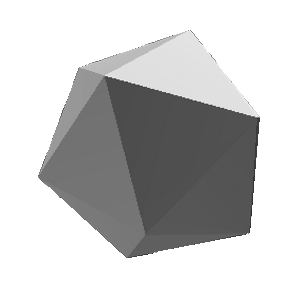
\includegraphics[width=0.25\textwidth]{img/sph_0.png}}   \hspace{.0\textwidth}
	\subfloat[960]  {\label{fig:sph2}   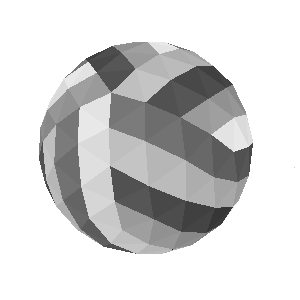
\includegraphics[width=0.25\textwidth]{img/sph_2.png}}   \hspace{.0\textwidth}
	\subfloat[61440]{\label{fig:sph5}   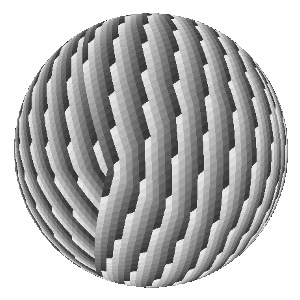
\includegraphics[width=0.25\textwidth]{img/sph_5.png}}   \hspace{.0\textwidth} \\
	\subfloat[4]    {\label{fig:sph_def}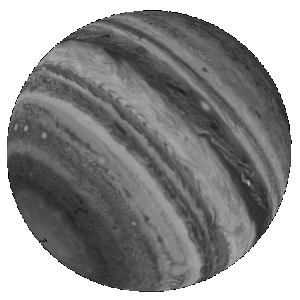
\includegraphics[width=0.25\textwidth]{img/sph_def.png}} \hspace{.0\textwidth} 
\caption{Porównanie wyglądu planet i ilości wierzchołków}
\label{fig:geom}
\end{figure}

\paragraph{}

U podstaw pomysłu na zredukowanie ilości wierzchołków do czterech leży spostrzeżenie że tak naprawdę kula wygląda z każdej strony dokładnie tak samo. Ponieważ siatki trójkątów nie korzystają z tego faktu, i dość kiepsko radzą sobie z płynnymi powierzchniami, kula staje się dla nich bardzo trudnym obiektem. Jeśli by natomiast generować geometrię kuli w inny sposób, dało by się bardzo wiele zaoszczędzić.

\paragraph{}

Jak już ustaliliśmy, dla wygenerowania finalnego obrazu potrzebne nam są przede wszystkim pozycja i normalna powierzchni w danym pikselu. Reszta danych zawartych w buforze geometrii jest stała dla planety i można ją otrzymać w oczywisty sposób. Jedynym wyjątkiem jest teksturowanie, które jednak zostanie opisane w rozdziale \hyperref[sub:nakladanie tekstur]{\ref{sub:nakladanie tekstur}}. Pozycje powierzchni planety jesteśmy w stanie łatwo obliczyć posiadając pozycję środka planety, oraz normalną planety w danym pikselu, według wzoru:

\begin{equation} \label{eq:pos}
pozycja = normalna \cdot promien + srodek\_planety
\end{equation}

Potrzebujemy więc otrzymać jedynie normalną w danym pikselu i będziemy mogli skonstruować cały bufor geometrii. Pomysł na wygenerowanie geometrii kuli, polega na stworzeniu dwuwymiarowej mapy normalnych kuli, następnie wstawieniu jej w odpowiednie miejsce w buforze geometrii. Najlepszym sposobem na stworzenie takiego bufora z mapami normalnych, jest wyświetlenie kwadratów w miejscach planet, o boku długości średnic planet, oraz oteksturowanie ich mapą normalnych. W ten sposób to OpenGL będzie odpowiedzialny za skalowanie, clipping, oraz wyświetlenie planety w odpowiednim miejscu. Teksturowanie również należy do banalnych czynności wykonywanych przez bibliotekę graficzną. Fragment shader będzie potrzebny do policzenia pozycji powierzchni planety z normalnej, według wzoru \hyperref[eq:pos]{\ref{eq:pos}}.

\paragraph{}

\begin{figure}
\centering
	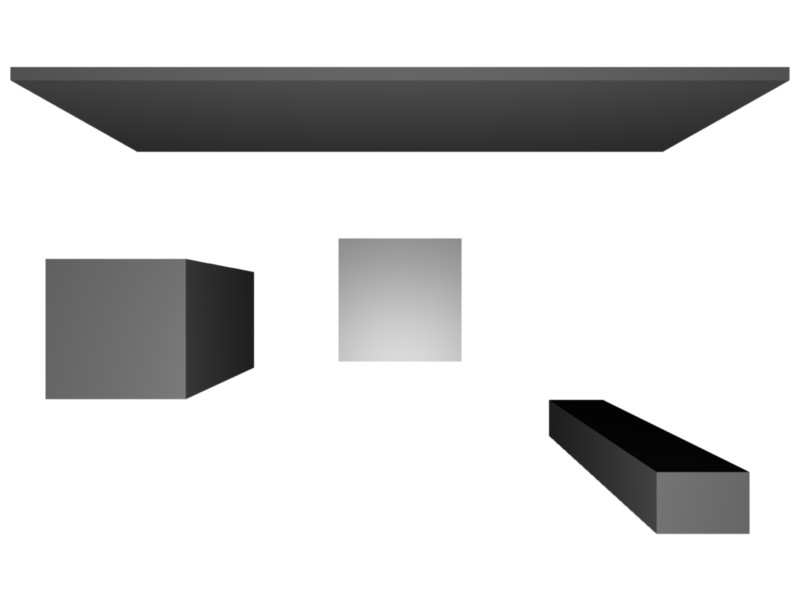
\includegraphics[width=0.5\textwidth]{img/proj_rend.jpg}
\caption{Rzut perspektywiczny sześcianów}
\label{fig:proj}
\end{figure}

Powyższy algorytm byłby prawdziwy, gdyby zastosowany został rzut ortogonalny. Ponieważ jednak w symulacjach o wiele bardziej naturalny jest rzut perspektywiczny, należy przystosować do niego powyższy algorytm. W rzucie perspektywicznym, jak pokazane na obrazku \hyperref[fig:proj]{\ref*{fig:proj}}, w zależności od pozycji obiektu względem kamery, może być widoczny z różnych stron. Dodatkowo obiekty znajdujące się na brzegu kamery ulegają zniekształceniu z powodu dystorsji. Aby realistycznie oddać rzut perspektywiczny należy uwzględnić te dwa efekty. Dystorsję obiektywu można uzyskać poprzez obrócenie kwadratów na które nakładana jest mapa normalnych, tak aby zwrócone były w stronę kamery. Oznacza to że normalna powierzchni dowolnego kwadratu, jest równoległa do prostej łączącej środek kwadratu (pozycję planety) z pozycją kamery. W ten sposób kwadraty te zostaną przekształcone macierzą projekcji, tak że będą w miarę realistycznie oddawać zniekształcenia obiektywu. Drugim problemem są źle obrócone normalne. Jedynym wyjściem jest dla każdej normalnej, obrócenie jej tak aby była poprawna. Obrót ten musi zostać wykonany o taki sam kąt, o jaki obrócony został kwadrat danej planety. Ponieważ obydwa te obroty są dokładnie takie same, wystarczy dla każdej planety skonstruować jedną macierz rotacji i przemnożyć przez nią zarówno normalne, jak i wektory tworzące kwadrat planety.

% Wstawić wynik renderowania normalny? Wymaga to niestety koloru:/

\paragraph{}

Dodatkowo do mapy normalnych należy dodać informację o przezroczystości danego obszaru. Dzięki temu, rogi kwadratu wyświetlającego planetę, będą mogły być przezroczyste. Planeta będzie miała więc przezroczystość ustawioną na 1.0 lub 0.0. Podczas renderowania, wszystkie piksele których przezroczystość jest mniejsza od ustalonej wartości (np. 0.1) nie zostaną wyświetlone. Sprawi to że wyświetlane kwadraty będą wyglądały jak koła, a po dodaniu oświetlenia i tekstur, staną się ładnymi kulami.

\subsection{Obliczanie oświetlenia}\label{sub:obliczanie oświetlenia}
\paragraph{}

\begin{figure}
\centering
	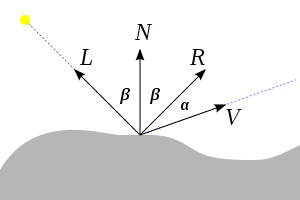
\includegraphics[width=0.5\textwidth]{img/phong.png}
\caption{Model oświetlenia Phonga}
\label{fig:phong}
\end{figure}

Do obliczania oświetlenia wykorzystany w programie został model Phonga. Polega on na złożeniu czterech rodzai świateł: emisji (emissive), otoczenia (ambient), rozproszonego (diffuse) i odbitego (specular). Jak pokazano na obrazku \hyperref[fig:phong]{\ref*{fig:phong}}, do obliczenia oświetlenia w danym punkcie potrzebne są: pozycja kamery, pozycja powierzchni, normalna powierzchni. Resztę potrzebnych wektorów da się obliczyć na podstawie tych trzech danych. Dla jednego źródła światła, model oświetlenie można zapisać jako:


$$ I = k_e I_e + k_a I_a + k_d I_d + k_s I_s = k_e I_e + k_a I_a + I_i( k_d( N \cdot L ) + k_s ( R \cdot V )^n ) $$

Gdzie $k_x$ są współczynnikami danymi w materiale, natomiast $I_x$ są natężeniami poszczególnych rodzai światła. Natężenia $I_e$ oraz $I_a$ są zadane arbitralnie dla całej sceny takie same. W naszym programie ustaliliśmy je na $1$, w ten sposób pełne sterowanie natężeniem światła otoczenia i emisji, zależą od współczynników. Natężenie $I_i$ zależy zazwyczaj od odległości powierzchni od źródła światła. W rzeczywistości światło zanika kwadratowo wraz z odległością, jednak my zdecydowaliśmy się zastosować wygaszanie liniowe, ponieważ czysto subiektywnie wydaje nam się że sceny z takim światłem wyglądają lepiej. W pierwszej implementacji, zawarte były wszystkie rodzaje świtała z modelu Phonga, jednak w końcu zdecydowaliśmy się na usunięcie z modelu oświetlenia światła odbitego. W efekcie model oświetlenia można zapisać jako:

$$ I = k_e I_e + k_a I_a + k_d I_d = k_e I_e + k_a I_a + I_i k_d( N \cdot L ) $$

Wpływ na taką decyzję miały dwa czynniki. Pierwszym było to, że praktycznie wszystkie materiały których używaliśmy, wyglądały najlepiej z minimalnym wpływem światła odbitego, lub w ogóle bez niego. W rzeczywistości faktycznie planety rzadko kiedy mają gładkie powierzchnie odbijające promienie światła jak szkło lub metal. Jednak decydujący wpływ na usunięcie tego oświetlenia miało dodanie atmosfer. Okazało się że po dodaniu koloru atmosfery, potrzebne jest 17 pozycji w buforze geometrii. Dodanie kolejnej tekstury wynikowej znacząco spowolniło by wyświetlanie, więc kosztem i tak nie bardzo używanego $k_s$ wszedł jeden z kolorów atmosfery. Zabieg ten nawet przyśpieszył trochę silnik graficzny, ponieważ światło odbite jest najbardziej kosztowne w obliczeniach.

\paragraph{}

Finalny obraz oświetlonych planet, generowany jest poprzez dodanie do siebie wielu obrazów. Dzięki addytywności światłą, można oddzielnie wyrenderować obraz dla każdego źródła światłą, następnie nałożyć na siebie te obrazy, dodając wartości kolorów w każdym pikselu. Zupełnie oddzielny przebieg posiadają światła emisji oraz otoczenia. Dla obu tych świateł generowany jest jeden obraz. W pierwszej wersji oświetlenia, dla każdego źródła światła na scenie generowany był kwadrat na cały ekran, a następnie był na nim wyświetlany wynikowy obraz dla konkretnego, jednego, źródła światła. Po dodaniu tych obrazów powstawał końcowy obraz. Aktualnie oświetlenie zyskało dodatkową optymalizację. Cały bazowy pomysł nie uległ zmianie, natomiast nie są już wyświetlane pełnoekranowe kwadraty dla każdego źródła światła. Optymalizacja taka spowodowana jest tym, że można stworzyć na scenie dużo niezależnych galaktyk. W ten sposób nawet jeśli na scenie jest sto świateł, ale na aktualnie widziane planety wpływ mają tylko dwie, silnik będzie działał tak samo wydajnie, jak gdyby na scenie były tylko dwa światła. Zastosowana optymalizacja pozwala na płynne przemieszczanie się, w nawet bardzo dużych układach planetarnych, z dużą ilością słońc.

\subsection{Nakładanie tekstur}\label{sub:nakladanie tekstur}
\paragraph{}

Klasyczne podejście do nakładania tekstur przewiduje tworzenie mapy UV, zawierającą siatkę obiektu. Każdy trójkąt, który jest obiektem 2D, ma przypisany trójkąt z płaskiej tekstury. W ten sposób można nałożyć siatkę na obiekt 3D. Jednak w aktualnym podejściu do generowania geometrii nie ma trójkątów tworzących obiekt, nie ma więc prostego sposobu na stworzenie siatki obiektu. Pojawiła się więc konieczność znalezienia ciągłego sposobu mapowania płaszczyzny na kulę. Po kilku próbach znalezienia najlepszego mapowania, z pomocą przyszła geografia. Kartografowie od dawana zmagali się z problemem najlepszego przedstawienia kuli ziemskiej na płaszczyźnie. Okazało się że istnieją różne metody projekcji mapy, w zależności od zachowania jednej z podstawowych właściwości. Metody mapowania można podzielić na:
\begin{description}
\item[zachowanie kątów] -- mapa jest rzutem azymutalnym z zachowaniem szerokości i długości geograficzych
\item[zachowanie odległości] -- na takiej mapie można mierzyć odległości w każdym kierunku i nie będą się one zmieniać w zależności od długości bądź szerokości kuli
\item[zachowanie kierunków] -- mapy takie używane są w nawigacji, ponieważ zachowują kąty kursów niezależnie od długości geograficznej (\hyperref[fig:merc]{\ref{fig:merc}})
\item[zachowanie powierzchni] -- w każdym punkcie kuli ziemskiej można zmierzyć pole powierzchni (\hyperref[fig:sinus]{\ref{fig:sinus}})
\end{description}

\begin{figure}
\centering
	\subfloat[Mercator]{\label{fig:merc}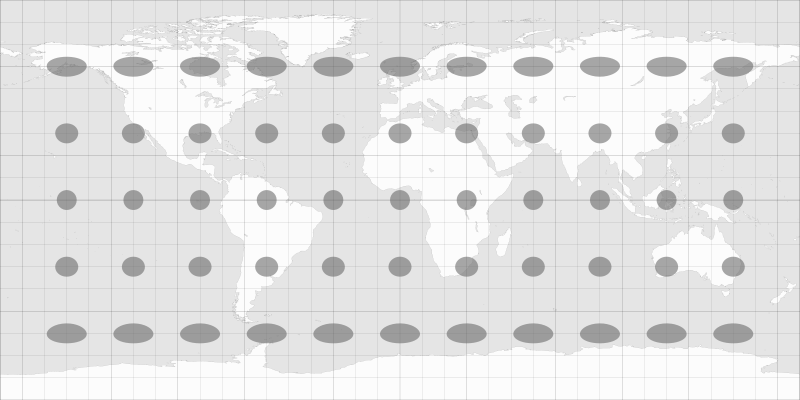
\includegraphics[width=0.45\textwidth]{img/proj_mer.png}} \hspace{.0\textwidth}
	\subfloat[Sinusoidalne]{\label{fig:sinus}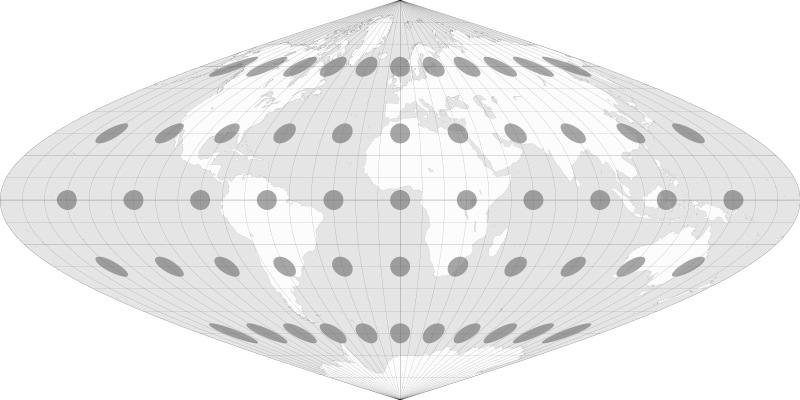
\includegraphics[width=0.45\textwidth]{img/proj_sin.png}}
\caption{Przykłady mapowania sfery}
\label{fig:project}
\end{figure}

Na ilustracji \hyperref[fig:project]{\ref{fig:project}}, pokazane są dwa mapowania które były przetestowane do teksturowania. Pierwszym jest mapowanie Mercatora, bardzo popularne ze względu na swoją przydatność w nawigacji. Ma również tą zaletę, że bardzo wiele tekstur planet udostępnianych w internecie jest zwykle właśnie w taki sposób mapowane. Okazało się jednak, że przeniesienie takiej mapy na kulę, choć prosta obliczeniowo, powoduje spore zniekształcenia ze względu na zaokrąglenia. W miejscach gdzie potrzebujemy mało pikseli na kuli, komputer musiał wybierać jeden z bardzo wielu dostępnych na mapie pikseli, w efekcie kula oteksturowana pikselami z brzegu mapy, wyglądała źle. Rozwiązaniem tego problemu było wybranie któregoś z mapowań zachowujących powierzchnię. Dzięki temu, można dobrze przeskalować obraz przed uruchomieniem programu, a następnie z mapowaniem nie ma już problemów. Najtańszym obliczeniowo sposobem, okazało się mapowanie sinusoidalne. Wymaga ono jedynie jednego $\cos$ do obliczenia. Z dokładnością do stałej, wzory na uzyskanie koordynat tekstury z szerokości i długości geograficznej w mapowaniu sinusoidalnym, przedstawiają się następująco:
\begin{eqnarray}
	u &=& \lambda cos(\phi) \\ \nonumber
	v &=& \phi
\end{eqnarray}
Jednak w trakcie obliczeń nie mamy jawnie podanych szerokości i długości geograficznej. Można łatwo policzyć te wartości, posiadając pozycję $(x,y,z)$ punktu na kuli.
\begin{eqnarray}\label{eq:texobj}
	\lambda &=& \arctan(\frac{z}{x}) \\ \nonumber
	\phi &=& \arcsin(\frac{y}{r}) = \arcsin(y) 
\end{eqnarray}
Obliczenia możemy prowadzić dla kuli o dowolnym promieniu. Wyniki będą jednak takie same dla każdej kuli, dlatego przyjęte zostało że teksturowana kula ma promień równy $1$. Wektor $(x,y,z)$ przedstawia punkt w przestrzeni obiektu, gdzie środkiem układu jest środek planety. Do tej pory wszystkie obliczenia graficzne prowadzone były w przestrzeni kamery, gdzie środkiem układu jest pozycja kamery. Mamy natomiast normalne kuli, które zero mają w środku planety, jednak obrócone są zawsze w stronę kamery. Musimy więc obrócić normalne. Obrót musi być obrotem przeciwnym do obrotu kamery. Wystarczy więc transponować macierz obrotu kamery, aby uzyskać pożądaną macierz.
\begin{eqnarray}
(x,y,z) &=& R \cdot N \\ \nonumber
R &=& R_k^T
\end{eqnarray}
Silnik graficzny nie udostępnia jednak jawnie macierzy obrotu kamery. Możemy natomiast bardzo łatwo uzyskać pełną macierz przekształcenia kamery $K$. Uzyskanie macierzy obrotu jest jednak banalne. Wiemy że kamera nie ulega skalowaniu. Jedyne przekształcenia to translacja i obrót. Macierz obrotu możemy więc łatwo uzyskać, wiedząc że dane o translacji zawarte są w dolnym rzędzie macierzy przekształcenia. Może więc napisać że:
\begin{eqnarray}
R_k &=&  
\left| \begin{array}{cccc}
K_{11} & K_{12} & K_{13} & 0 \\ 
K_{21} & K_{22} & K_{23} & 0 \\
K_{31} & K_{32} & K_{33} & 0 \\
0 & 0 & 0 & 1 
\end{array} \right|
\end{eqnarray}
Po takim obrocie normalnych, stają się one pożądanym wektorem $(x,y,z)$ ze wzoru \hyperref[eq:texobj]{\ref{eq:texobj}}, w przestrzeni obiektu, którym jest kula o promieniu równym $1$. Możemy więc zastosować podane wcześniej wzory, uzyskując końcowe koordynaty tekstury.

\subsection{Atmosfery}\label{sub:atmosfery}
\paragraph{}

Ogólny problem renderowania atmosfery jest problemem niebanalnym. Najlepsze implementacje polegają na pewniej formie raytracingu i sprawdzają się dla realistycznych symulacji ziemi. Taka symulacja przewiduje jedną planetę i jedno słońce. W naszej sytuacji byliśmy zmuszeni do pewnych ustępstw, ponieważ priorytetem jest zachowanie czasu rzeczywistego symulacji. Przede wszystkim, nasze planety są zawsze widoczne z daleka. Można więc nie zawracać sobie głowy zbliżeniami wchodzącymi w atmosferę i lądującymi na powierzchni ziemi. Samo to jednak nie upraszcza modelu wystarczająco.

\paragraph{}

Po kilku próbach zdecydowaliśmy że modelem łączącym szybkość działania, z w miarę realistycznym wyglądem, będzie nakładanie na kule dodatkowej półprzezroczystej warstwy atmosfery. Kolor będzie modulowany analogicznie do modelu oświetlenia Phonga, z tą różnicą, że atmosfery będą oświetlane trochę głębiej niż normalna kula. Kule już w połowie stają się zupełnie ciemne, w przypadku atmosfer jest inaczej. Z powodu półprzezroczystości, światło sięga dalej i oświetla górną część atmosfery. Efekt ten, pokazany jest na obrazku \hyperref[fig:atmo]{\ref{fig:atmo}}. Pogrubioną linią zaznaczona jest oświetlona część atmosfery. Aby podobnie oświetlić atmosferę, zdecydowaliśmy się tylko lekko zmodyfikować model oświetlenia pokazany w rozdziale \hyperref[sub:obliczanie oświetlenia]{\ref{sub:obliczanie oświetlenia}}.
\begin{eqnarray}
I_d = I_i k_d( N \cdot L + const )
\end{eqnarray}
Gdzie $const$ oznacza stałą, wzmacniającą oświetlenie atmosfery. Dzięki temu tam gdzie planeta staje się już zupełnie czarna, atmosfera jest dalej nakładana. Efekt takiego zabiegu okazał się zadowalający, a co najważniejsze jest dość tani obliczeniowo.


\begin{figure}
\centering
	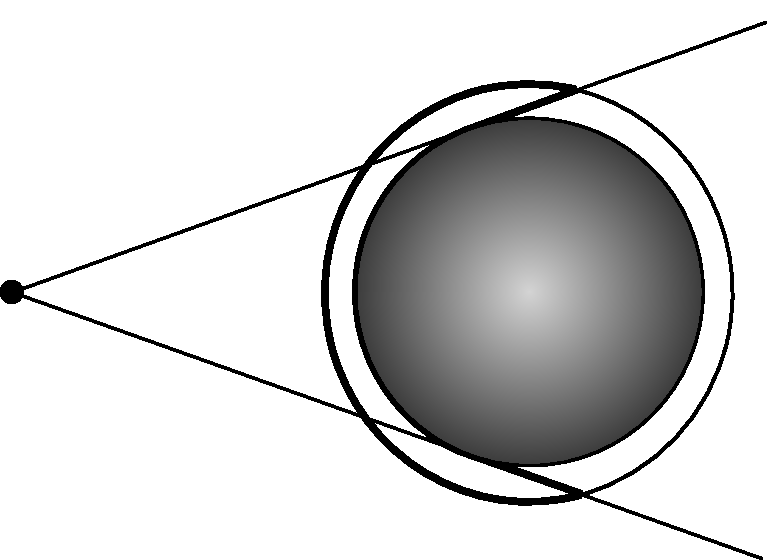
\includegraphics[width=0.5\textwidth]{img/atm.pdf}
\caption{Oświetlenie atmosfery}
\label{fig:atmo}
\end{figure}

\paragraph{}

Technicznie, atmosfery do wyświetlenia potrzebują swoich dwóch przebiegów. Aby wykorzystać już obliczany iloczyn skalarny wprowadzona została również zmiana w bazowym przebiegu. W tym przebiegu, do koloru planety po nałożeniu tekstur, dodawany jest kolor atmosfery. Uzyskuje się w ten sposób wygląd półprzezroczystej atmosfery, pokrywającej planetę, jednak nie mającej żadnej grubości, ponieważ nic nie wystaje za planetę. Ponieważ deferred rendering nie pozwala na przezroczystości, w celu wyświetlenia atmosfer poza planetami, potrzebne są dodatkowe dwa przebiegi. Działają one analogicznie do przebiegów rysujących planety, z tą różnicą, że mapa normalnych wygląda inaczej. Normalne atmosfery są efektywnie rzutem normalnych kuli na płaszczyznę, czyli mają składową $z$ równą $0$. Wartość $\alpha$ jest natomiast coraz mniejsza im dalej od środka tekstury. Oświetlenie takiej mapy normalnych daje ładne wyniki na brzegu tekstury, dlatego służy ona do wyświetlania półprzezroczystej obwódki planet. Środek planety ciągle wyświetlany jest pierwszymi przebiegami. Płaszczyzny atmosfer są cofnięte względem środka planety, a do drugiego przebiegu wykorzystywane jest zbuffor powstały po przebiegu rysowania planet. Dzięki temu wyświetlany jest tylko brzeg atmosfer i szczelnie przylega on do wcześniej wyświetlonych planet. Końcowy efekt jest zadowalający nawet na sporych zbliżeniach.

